%
% File tensorfactor.tex
%%
%% Based on the style files for COLING-2014, which were, in turn,
%% Based on the style files for ACL-2014, which were, in turn,
%% Based on the style files for ACL-2013, which were, in turn,
%% Based on the style files for ACL-2012, which were, in turn,
%% based on the style files for ACL-2011, which were, in turn, 
%% based on the style files for ACL-2010, which were, in turn, 
%% based on the style files for ACL-IJCNLP-2009, which were, in turn,
%% based on the style files for EACL-2009 and IJCNLP-2008...

%% Based on the style files for EACL 2006 by 
%%e.agirre@ehu.es or Sergi.Balari@uab.es
%% and that of ACL 08 by Joakim Nivre and Noah Smith

\documentclass[11pt]{article}
\usepackage{coling2016}
\usepackage{uarial}
\usepackage{url}
\usepackage{listings}
\usepackage{graphicx}
\usepackage[fleqn]{amsmath}
\usepackage{amssymb}

\usepackage{placeins}
\usepackage{latexsym}
\usepackage{hyperref}
\usepackage{wrapfig}
\usepackage{algorithm}
\usepackage{algorithmic}

\title{Matrix/Tensor Factorization}

\author{
  \textbf{Madhav Datt} \\
  Indian Institute of Technology, Kharagpur \\
  \texttt{madhav$@$iitkgp.ac.in}
}


\begin{document}
\maketitle
\begin{abstract}
Matrix and tensor factorization is a group of algorithms and techniques in multivariate analysis. We especially explore non-negative matrix and tensor factorization (NMF and NTF) which, even though is a significantly more challenging problem, has greater applicability. The nonnegativity constraints have been shown to enable natural interpretations and allow better solutions in numerous applications including image processing, text analysis, and bioinformatics. However, the computation of NMF and NTF is a NP-hard problem in general, and remains challenging and expensive due the constraints. Numerous algorithmic approaches have been proposed to efficiently compute NMF and NTF. In this extremely brief survey paper, we start by defining the NMF problem, along with discussing classical approaches, such as alternating least squares, for solution estimation, both from an intuitive and a rigorous mathematical perspective. We survey some of the state of the art numerical methods and algorithms for NMF. Further, we compare these methods and examine their advantages and disadvantages in terms of convergence to optimum values, loss minimization, algorithmic efficiency etc. We also look at modifications to enable these algorithms to handle very large-scale data. Finally, we briefly describe some problems and applications in image processing where non-negative matrix and tensor factorization finds very direct use.
\end{abstract}

\section{Introduction}
In this brief and introductory survey, we explore Matrix and Tensor Factorization, which is a group of algorithms in multivariate analysis and linear algebra where a matrix $\mathbf{V}$ is, usually, though not always, factorized into two matrices $\mathbf{W}$ and $\mathbf{H}$. In text mining, signal processing, image processing, and computer vision among other areas, imposing non-negativity constraints to the low-rank factors of matrices (ie. $w \geq 0, h \geq 0 ~ \forall ~ w \in \mathbf{W}, h \in \mathbf{H}$) and tensors has been shown an effective technique providing physically meaningful interpretations of the signal or image data involved, and is inherent to the data.  For example, in image processing and computer vision, involved variables and parameters may correspond to pixels, and nonnegative sparse decomposition is related to the extraction of relevant parts from the images as shown in works \cite{93}, \cite{94}. Since this problem is not exactly solvable in general, it is commonly approximated through various numerical methods and algorithms.

In the rest of this paper, we focus on discussions and analysis state-of-the-art algorithms for non-negative matrix or tensor factorization (NMF) \cite{113}, and explore some of its applications to image processing.

\subsection{Basic NMF Model}
The basic NMF problem can formally be defined and stated as follows: Given a nonnegative data matrix $\mathbf{Y} \in \mathbb{R}^{I \times T}_{+}$
(with $y_{it} \geq 0$ or equivalently $\mathbf{Y} \geq 0$) and a reduced rank $\mathit{J}$ ($\mathit{J} \leq \min(I, T)$), find two nonnegative matrices $\mathbf{A} = [\mathbf{a}_1, \mathbf{a}_2, \dots , \mathbf{a}_J ] \in \mathbb{R}^{I \times J}_{+}$
and $X = B^T = [\mathbf{b}_1, \mathbf{b}_2, \dots , \mathbf{b}_J]^T
\in \mathbb{R}^{J \times T}_{+}$ which factorize $\mathbf{Y}$ as well as possible, that is
$$\mathbf{Y} = \mathbf{A}\mathbf{X} + \mathbf{E} = \mathbf{A}\mathbf{B}^T + \mathbf{E}$$
where the matrix $\mathbf{E} \in \mathbb{R}^{I \times T}$ represents approximation error. The factors $\mathbf{A}$ and $\mathbf{X}$ may have different physical meanings in different applications, and are assumed to be non-negative in standard NMF.

The NMF model can also be represented as a special form of the bilinear model, as follows:
$$\mathbf{Y} = \sum_{j=1}^J \mathbf{a}_j \circ \mathbf{b}_j + \mathbf{E} = \sum_{j=1}^J \mathbf{a}_j \mathbf{b}_j^T + \mathbf{E}$$

where the symbol $\circ$ denotes the outer product of two vectors. Thus, we can build an approximate representation of the nonnegative data matrix $\mathbf{Y}$ as a sum of rank-one nonnegative matrices $\mathbf{a}_j\mathbf{b}_j^T$. If such decomposition is exact (i.e., $\mathbf{E} = 0$) then it is called the Nonnegative Rank Factorization (NRF) \cite{53}. Among the many possible series representations of data matrix $\mathbf{Y}$ by nonnegative rank-one matrices, the smallest integer $\mathit{J}$ for which such a nonnegative rank-one series representation is attained is called the nonnegative rank of the nonnegative matrix $\mathbf{Y}$ and
it is denoted by $rank_+(\mathbf{Y})$. The nonnegative rank satisfies the following bounds, as shown by \cite{53}:
$$rank(\mathbf{Y}) \leq rank_+(\mathbf{Y}) \leq \min(I, T)$$

\FloatBarrier
\begin{figure}[!htbp]
\centering
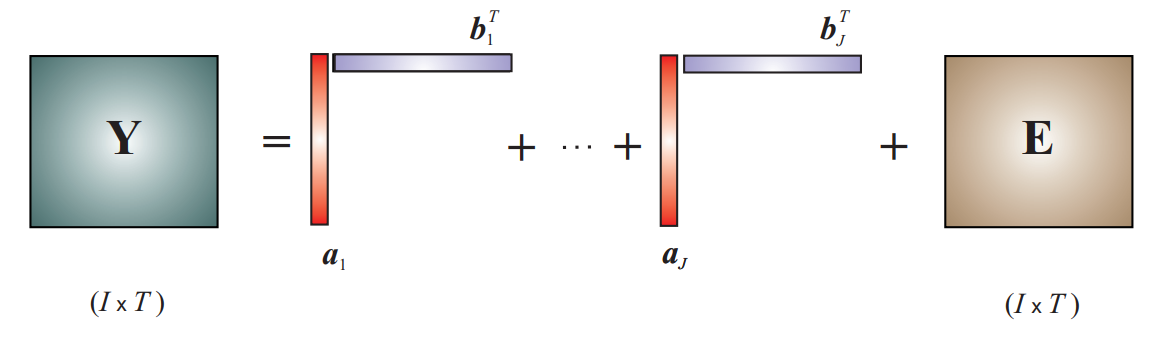
\includegraphics[width=0.9\textwidth]{bilinear}
\caption{Bilinear NMF model. The nonnegative data matrix $\mathbf{Y} \in \mathbb{R}^{I \times T}_{+}$ is approximately represented by a sum or linear combination of rank-one nonnegative matrices $\mathbf{Y}^{(j)} = \mathbf{a}_j \circ \mathbf{b}_j = \mathbf{a}_j \mathbf{b}_j^T \in \mathbb{R}^{I \times T}_{+}$.} 
\label{fig1}
\end{figure}
\FloatBarrier

\blfootnote{Figures \ref{fig1} and \ref{fig2} are based on explanations and figures provided in \cite{p22}.}

An NMF is not necessarily an NRF in the sense that the latter demands the exact factorization whereas the former is usually only an approximation. In many applications we require additional constraints on the elements of matrices $\mathbf{A}$ and/or $\mathbf{X}$, such as smoothness, sparsity, symmetry, and
orthogonality, the discussion of which is beyond the scope of this paper.

\subsection{Basic Approaches to Parameter Estimation}

In order to estimate factor matrices $\mathbf{A}$ and $\mathbf{X}$ in the standard NMF, we need to consider the similarity measure to quantify a difference between the data matrix $\mathbf{Y}$ and the approximative NMF model matrix $\hat{\mathbf{Y}} = \mathbf{AX}$. The choice of the similarity measure (also referred to as distance, divergence or measure of dissimilarity) mostly depends on the probability distribution of the estimated signals or components and on the structure of data or a distribution of noise. The
simplest and most often used measure is based on Frobenius norm:
$$D_F(\mathbf{Y}||\hat{\mathbf{Y}}) = \frac{1}{2}||\mathbf{Y-AX}||_F^2$$

which is also referred to as the squared Euclidean distance. It should be noted that the above cost function is convex with respect to either the elements of the matrix $\mathbf{A}$ or the matrix $\mathbf{X}$, but not both. Another frequently used cost function for NMF is the generalized Kullback-Leibler divergence, as shown in \cite{94}, (also called the I-divergence):
$$D_{KL}(\mathbf{Y}||\hat{\mathbf{Y}}) = \sum_{it} \left( y_{it} \ln \frac{y_{it}}{[\mathbf{AX}]_{it}} - y_{it} + [\mathbf{AX}]_{it} \right)$$

Alternating minimization of such a cost leads to the ALS (Alternating Least Squares)
algorithm which is a fixed point algorithm, where each iteration can be described as follows:

\begin{enumerate}
\item  Initialize $\mathbf{A}$ randomly or by using a specific deterministic strategy.
\item Estimate $\mathbf{X}$ from the matrix equation $\mathbf{A}^T\mathbf{AX} = \mathbf{A}^T\mathbf{Y}$ by solving
$$\min_X D_F(\mathbf{Y} || \mathbf{AX}) = \frac{1}{2} ||\mathbf{Y-AX}||_F^2 \textrm{ with fixed } \mathbf{A}.$$
\item Set all the negative elements of $\mathbf{X}$ to zero or some small positive value $\epsilon$.
\item Estimate $\mathbf{A}$ from the matrix equation $\mathbf{XX}^T\mathbf{A}^T = \mathbf{XY}^T$ by solving
$$\min_A D_F(\mathbf{Y} || \mathbf{AX}) = \frac{1}{2} ||\mathbf{Y}^T-\mathbf{X}^T\mathbf{A}^T||_F^2 \textrm{ with fixed } \mathbf{X}.$$
\item Set all the negative elements of $\mathbf{A}$ to zero or some small positive value $\epsilon$.
\end{enumerate}

It is possible to rewrite the above algorithm into a more concise form as the following iterative, fixed point algorithm update statements:

\begin{eqnarray}
\mathbf{X} \leftarrow \max(\epsilon, (\mathbf{A}^T\mathbf{A})^{-1}\mathbf{A}^T\mathbf{Y}) = [\mathbf{A}^{\dagger}\mathbf{Y}]_+ \\
\mathbf{A} \leftarrow \max(\epsilon, \mathbf{YX}^T(\mathbf{XX}^T)^{-1}) = [\mathbf{YX}^{\dagger}]_+
\end{eqnarray}

where, the $\dagger$ symbol denotes the Moore-Penrose inverse of the matrix, and $\epsilon$ is a very small constant (typically in the order of $10^{-16}$) to enforce positive entries in the resulting matrices.

The above described ALS method is considered as a basic "workhorse" approach, however it is not
guaranteed to converge to a global minimum nor even a stationary point, but only to a solution
where the cost functions cease to decrease (\cite{85}, \cite{11}). Moreover, it is often not sufficiently accurate. The ALS method can be dramatically improved and its computational complexity reduced with algorithms and methods that are discussed in the next section on State of the art Algorithms.

\section{State of the art Algorithms}
In this section, we discuss some of the most effective state-of-the-art algorithms and numerical methods for matrix and tensor factorization. Further, we examine and compare all the discussed algorithms based on their advantages and disadvantages. Before we go into the discussion on NMF algorithms, we provide a brief and intuitive note on large scale NMF methods, which are particularly relevant to image processing, and how these can be applied in case of the algorithms discussed below.

\subsection{Large-Scale NMF}
In many image processing applications, especially in dimension reduction applications the data matrix $\mathbf{Y} \in \mathbb{R}^{I \times T}$ can be very large (with millions of entries), but it can be approximately factorized using a rather smaller number of nonnegative components ($\mathit{J}$), that is, $\mathit{J} << I$ and $\mathit{J} << T$. Then the problem $\mathbf{Y} \approx \mathbf{AX}$ becomes highly redundant and we do not need to use information about all entries of $\mathbf{Y}$ in order to estimate precisely the factor matrices $\mathbf{A} \in \mathbb{R}^{I \times J}$ and $\mathbf{X} \in \mathbb{R}^{J \times T}$. In other words, to solve the large-scale NMF problem we do not need to know the whole data matrix but only a small random part of it. In this approach, instead of performing large-scale factorization $$\mathbf{Y} = \mathbf{AX} + \mathbf{E}$$
we can consider a two set of linked factorizations using much smaller matrices, given by
\begin{eqnarray*}
\mathbf{Y}_r = \mathbf{A}_r\mathbf{X} + \mathbf{E}_r, \quad \textrm{for fixed and known } \mathbf{A}_r \\
\mathbf{Y}_c = \mathbf{A}\mathbf{X}_c + \mathbf{E}_c, \quad \textrm{for fixed and known } \mathbf{X}_c
\end{eqnarray*}
where $\mathbf{Y}_r \in \mathbb{R}^{R \times T}_+$ and $\mathbf{Y}_c \in \mathbb{R}^{I \times C}_+$ are the matrices constructed from the selected rows and columns of the matrix $\mathbf{Y}$, respectively. Analogously, we can construct the reduced matrices: $\mathbf{A}_r \in \mathbb{R}^{R \times J}$ and $\mathbf{X}_c \in \mathbb{R}^{J \times C}$ by using the same indices for the columns and rows as those used for the construction of the data sub-matrices $\mathbf{Y}_c$ and $\mathbf{Y}_r$. \cite{66}, \cite{15} discuss several strategies to choose the columns and rows of the input data matrix, where the simplest scenario is to choose the first $R$ rows and the first C columns of the data matrix as shown in Figure \ref{fig2}.

\begin{figure}[!htbp]
\centering
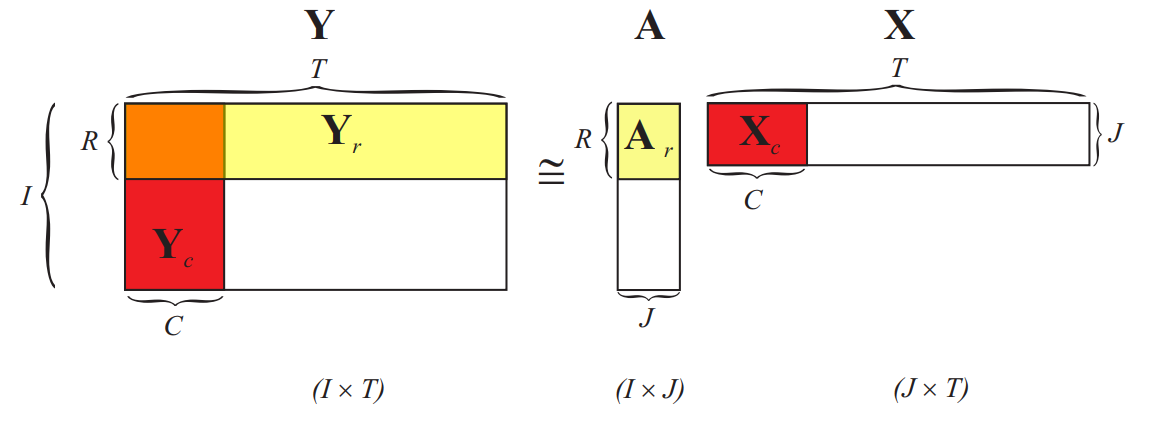
\includegraphics[width=0.9\textwidth]{large_scale}
\caption{Conceptual illustration of block-wise data processing for large-scale NMF. Instead of
processing the whole matrix $\mathbf{Y} \in \mathbb{R}^{I \times T}$, we can process much smaller block matrices $\mathbf{Y}_r \in \mathbb{R}^{R \times T}$ and $\mathbf{Y}_c \in \mathbb{R}^{I \times C}$ and corresponding factor matrices $\mathbf{A}_r \in \mathbb{R}^{R \times J}$ and $\mathbf{X}_c \in \mathbb{R}^{J \times C}$ with $C << T$ and $R << I$.}
\label{fig2}
\end{figure}
\FloatBarrier

\subsection{Two-Block Coordinate Descent Framework}
Almost all NMF algorithms designed, including the "workhorse" alternating least squares algorithm discussed in Section 1.2  use a two-block coordinate descent scheme, that is, they optimize alternatively over one of the two factors, $\mathbf{W}$ or $\mathbf{H}$, while keeping the other fixed. The reason is that the subproblem in one factor is convex. More precisely, it is a nonnegative least squares problem (NNLS): for example, for $\mathbf{H}$ fixed, we have to solve 
%\[
$$\min_{\mathbf{W} \geq 0} ||\mathbf{X-WH}||_F^2$$ 
%\]
Note that this problem has a particular structure as it can be decomposed into $p$ independent NNLS in $r$ variables since 
\begin{equation} \label{sepr}
||\mathbf{X-WH}||_F^2  
= \sum_{i=1}^p  ||\mathbf{X}_{i:}-\mathbf{W}_{i:}\mathbf{H}||_2^2
= \sum_{i=1}^p \mathbf{W}_{i:} \left(\mathbf{HH}^T\right) \mathbf{W}_{i:}^T - 2  \mathbf{W}_{i:} \left(\mathbf{HX}_{i:}^T\right) + ||\mathbf{X}_{i:}||_2^2. 
\end{equation}

Many algorithms exist to solve the NNLS problem, and NMF algorithms based on two-block coordinate descent differ by which NNLS algorithm is used. A comparative study based on the advantages and disadvantages of these NNLS algorithms is provided in section \ref{comp}. The general framework for these NMF algorithms to update $\mathbf{W}$ and $\mathbf{H}$ is given by the following algorithms.

\FloatBarrier
\renewcommand{\thealgorithm}{BCD}
\algsetup{indent=2em}
\begin{algorithm}[ht!]
\caption{Two-Block Coordinate Descent -- Framework of Most NMF Algorithms \label{nmfalgo}}
\begin{algorithmic}[1] 
\REQUIRE Input nonnegative matrix $\mathbf{X} \in \mathbb{R}^{p \times n}_+$ and factorization rank $r$. 
\ENSURE $(\mathbf{W,H}) \geq 0$: A rank-$r$ NMF of $\mathbf{X} \approx \mathbf{WH}$. 
    \medskip  
\STATE Generate some initial matrices $\mathbf{W}^{(0)} \geq 0$ and $\mathbf{H}^{(0)} \geq 0$; 
\FOR {$t$ = 1, 2, \dots }  
 \STATE  $\mathbf{W}^{(t)}$ = update$\left(\mathbf{X}, \mathbf{H}^{(t-1)}, \mathbf{W}^{(t-1)}\right)$. 
 \STATE  ${\mathbf{H}^{(t)}}^T$ = update$\left(\mathbf{X}^T,  {\mathbf{W}^{(t)}}^T, {\mathbf{H}^{(t-1)}}^T\right)$. 
\ENDFOR
\end{algorithmic}  
\end{algorithm} 
\FloatBarrier

\subsection{First-Order Optimality Conditions (Stationary Points)} 
Given $\mathbf{X}$, let us denote $F(\mathbf{W,H}) = \frac{1}{2}||\mathbf{X-WH}||_F^2$. The first-order optimality conditions for equations 1, 2 are
\begin{eqnarray}  
\mathbf{W} \geq 0, & \quad \nabla_{\mathbf{W}} F = \mathbf{WHH}^T - \mathbf{XH}^T \geq 0, & \quad \mathbf{W} \circ \nabla_{\mathbf{W}} F = 0, \label{kktc} \\
 \mathbf{H} \geq 0, & \quad \nabla_{\mathbf{H}} F = \mathbf{W}^T\mathbf{WH} - \mathbf{W}^T\mathbf{X} \geq 0, & \quad \mathbf{H} \circ \nabla_{\mathbf{H}} F = 0, \nonumber 
\end{eqnarray}
where $\circ$ is the component-wise product of two matrices. 
Any $(W,H)$ satisfying these conditions is a stationary point of equations 1 and 2 shown in section 1.2. 

\subsection{Multiplicative Updates} \label{mu}

Given $\mathbf{X}$, $\mathbf{W}$ and $\mathbf{H}$, the multiplicative updates (MU) modify $\mathbf{W}$ as follows 
\begin{equation} \tag{MU} 
\label{mup}
\mathbf{W} \leftarrow \mathbf{W} \circ \frac{\left[\mathbf{XH}^T\right]}{\left[\mathbf{WHH}^T\right]}
\end{equation}
where $\frac{[\,]}{[\,]}$ denotes the component-wise division between two matrices. The MU were first developed in~\cite{DM86} for solving NNLS problems, and later rediscovered and used for NMF in~\cite{94}. 
The MU are based on the majorization-minimization framework. In fact, \eqref{mup} is the global minimizer of a quadratic function majorizing $F$, that is, a function that is larger than $F$ everywhere and is equal to $F$ at the current iterate \cite{DM86} \cite{94}. Hence minimizing that function guarantees $F$ to decrease and therefore leads to an algorithm for which $F$ monotonically decreases. 
The MU can also be interpreted as a rescaled gradient method: in fact, 
\begin{eqnarray} \label{mugrad}
\mathbf{W} \circ \frac{\left[\mathbf{XH}^T\right]}{\left[\mathbf{WHH}^T\right]} = \mathbf{W} -  \frac{\left[\mathbf{W}\right]}{\left[\mathbf{WHH}^T\right]} \circ  \nabla_{\mathbf{W}} F . 
\end{eqnarray}
Another more intuitive interpretation is as follows: we have that 
% \[
$$\frac{\left[\mathbf{XH}^T\right]_{ik}}{\left[\mathbf{WHH}^T\right]_{ik}} \geq 1 \quad \iff \quad \left(\nabla_{\mathbf{W}} F\right)_{ik} \leq 0.$$
% \] 
Therefore, in order to satisfy \eqref{kktc}, for each entry of $\mathbf{W}$, the MU either 
(i)~increase it if its partial derivative is negative,   
(ii)~decrease it if its partial derivative is positive,  or 
(iii)~leave it unchanged if its partial derivative is equal to zero. 

If an entry of $\mathbf{W}$ is equal to zero, the MU cannot modify it hence it may occur that an entry of $\mathbf{W}$ is equal to zero while its partial derivative is negative which would not satisfy \eqref{kktc}.  

\subsection{Alternating Nonnegative Least Squares} \label{anls}

Alternating nonnegative least squares (ANLS) is a class of methods where the subproblems in $\mathbf{W}$ and $\mathbf{H}$ are solved exactly, that is, the update for $\mathbf{W}$ is given by  
\begin{eqnarray*}
\mathbf{W}  \leftarrow  \textrm{argmin}_{\mathbf{W} \geq 0} ||\mathbf{X-WH}||_F .  
\end{eqnarray*} 
Many methods can be used to solve the NNLS $\textrm{argmin}_{\mathbf{W} \geq 0} ||\mathbf{X-WH}||_F$, and dedicated active-set methods have shown to perform very well in practice. Since each iteration of ANLS computes an optimal solution of the NNLS subproblem, each iteration of ANLS decreases the error the most among NMF algorithms following the framework described in Algorithm~\ref{nmfalgo}. However, each iteration is computationally more expensive, and more difficult to implement. 

\subsection{Hierarchical Alternating Least Squares} \label{hals}

Hierarchical alternating least squares (HALS) solves the NNLS subproblem using an exact coordinate descent method, updating one column of $W$ at a time. The optimal solutions of the corresponding subproblems can be written in closed form. In fact, the entries of a column of $W$ do not interact - see Equation~\eqref{sepr} - hence the corresponding problem can be decoupled into $p$ quadratic problems with a single nonnegative variable.  HALS updates $W$ as follows. 
For $\ell = 1, 2, \dots, r$: 
\begin{eqnarray*}
\mathbf{W}(:,\ell) & \leftarrow \textrm{argmin}_{\mathbf{W}(:, \ell) \geq 0} \Big\|\mathbf{X}-\sum_{k\neq \ell} \mathbf{W}(:,k)\mathbf{H}(k,:) - \mathbf{W}(:,\ell)\mathbf{H}(\ell,:) \Big\|_F  \\ 
\mathbf{W}(:,\ell) & \leftarrow \max \left(0,  \frac{\mathbf{XH}(\ell,:)^T -\sum_{k\neq \ell} \mathbf{W}(:,k) \left(\mathbf{H}(k,:) \mathbf{H}(\ell,:)^T\right)   }{ ||\mathbf{H}(\ell,:)||_2^2 } \right)
\end{eqnarray*} 

In the original HALS, each column of $\mathbf{W}$ is updated only once before updating $\mathbf{H}$. However, as for the MU, it can be sped up by updating $\mathbf{W}$ several times before updating $\mathbf{H}$, or selecting the entries of $\mathbf{W}$ to update following a Gauss-Southwell-type rule. HALS can also be generalized to other cost functions using Taylor expansion \cite{g83}.

\subsection{Comparative Study: Advantages and Disadvantages} \label{comp}
In this section, we compare some of the underlying key differences between various algorithms, and more importantly, broad categories of numerical methods used. A statistical analysis of the difference of performances of the above algorithms, and their expected behaviors can be found in section \ref{analysis} (Analysis and Conclusion). A main difference between the projected iterative methods and the active-set-like methods for the NLS problems (and thus the NMF problem, since the NLS algorithms are used as subroutines for non-negative matrix, and tensor factorization) lies in their convergence or termination. In projected iterative methods, a sequence of tentative solutions is generated so that an optimal solution is approached in the limit. In practice, one has to somehow stop iterations and return the current estimate, which might be only an approximation of the solution. In the active-set and active-set-like methods, in contrast, there is no concept of a limit point. Tentative solutions are generated with a goal of finding the optimal active and passive set partitioning, which is guaranteed to be found in a finite number of iterations since there are only a finite number of possible active and passive set partitionings. Once the optimal active and passive sets are found, the methods terminate. There are trade-offs of these behavior. While the projected iterative methods may return an approximate solution after a few number of iterations, the active-set and active-set-like methods only return a solution after they terminate. After the termination, however, the solution from the active-set-like methods is an exact solution only subject to numerical rounding errors while the solution from the projected iterative methods might be an approximate one.

Other approaches for solving the NLS problems can be considered as a subroutine for the NMF computation. \cite{p2} have studied an interior point Newton-like method, and \cite{p31} presented a sequential coordinate-wise method. Some observations about the NMF computation based on these methods as well as other methods are offered in \cite{p22}. \cite{p18} proposed an algorithm based on low-dimensional polytope approximation: Their algorithm is motivated by a geometrical interpretation of NMF that data points are approximated by a simplicial cone \cite{p27}.

More specifically, the MU became extremely popular mainly because 
	(i)~they are simple to implement\footnote{For example, in Matlab: \texttt{W = W.*(X*H')./(W*(H*H'))}. \label{fn2}}, 
	(ii)~they scale well and are applicable to sparse matrices\footnote{When computing the denominator $WHH^T$ in the MU, it is crucial to compute $HH^T$ first in order to have the lowest computational cost.}, 
	and 
	(iii)~they were proposed in the paper of Lee and Seung~\cite{93} which launched the research on NMF. However, the MU converge relatively slowly. HALS has been observed to converge much faster than the MU while having almost the same computational cost. On the other hand, HALS is, under some mild assumptions, guaranteed to converge to a stationary point. For the ANLS algorithm, because usually the initial guess $\mathbf{WH}$ is a poor approximation of $\mathbf{X}$, it does not make much sense to solve the NNLS subproblems exactly at the first steps of Algorithm~\ref{nmfalgo}, and therefore it might be profitable to use ANLS rather in a refinement step of a cheaper NMF algorithm (such as the MU or ALS). 

\section{Applications in Image Processing}
The reason why NMF has become so popular is because of its ability to automatically extract sparse and easily interpretable factors. In this section, we illustrate this property of NMF through its applications in image processing.

\subsection{Facial Feature Extraction}

Let each column of the data matrix $\mathbf{X} \in \mathbb{R}^{I \times T}_+$ be a vectorized gray-level image of a face, with the $(i, j)$th entry of matrix $\mathbf{X}$ being the intensity of the $i$th pixel in the $j$th face. NMF generates two factors $(\mathbf{W}, \mathbf{H})$ so that each image $\mathbf{X}(:, j)$ is approximated using a linear combination of the columns of $\mathbf{W}$; see Equation and Figure \ref{fig3} for an illustration. Since $\mathbf{W}$ is nonnegative, the columns of $\mathbf{W}$ can be interpreted as images (that is, vectors of pixel intensities) which we refer to as the basis images. As the weights in the linear combinations are nonnegative ($\mathbf{H} \geq 0$), these basis images can only be summed up to reconstruct each original image. Moreover, the large number of images in the data set must be reconstructed approximately with only a few basis images (in fact, $r$ is in general much smaller than $n$), hence the latter should be localized features (hence sparse) found simultaneously in several images.

\FloatBarrier
\begin{figure}[!htbp]
\centering
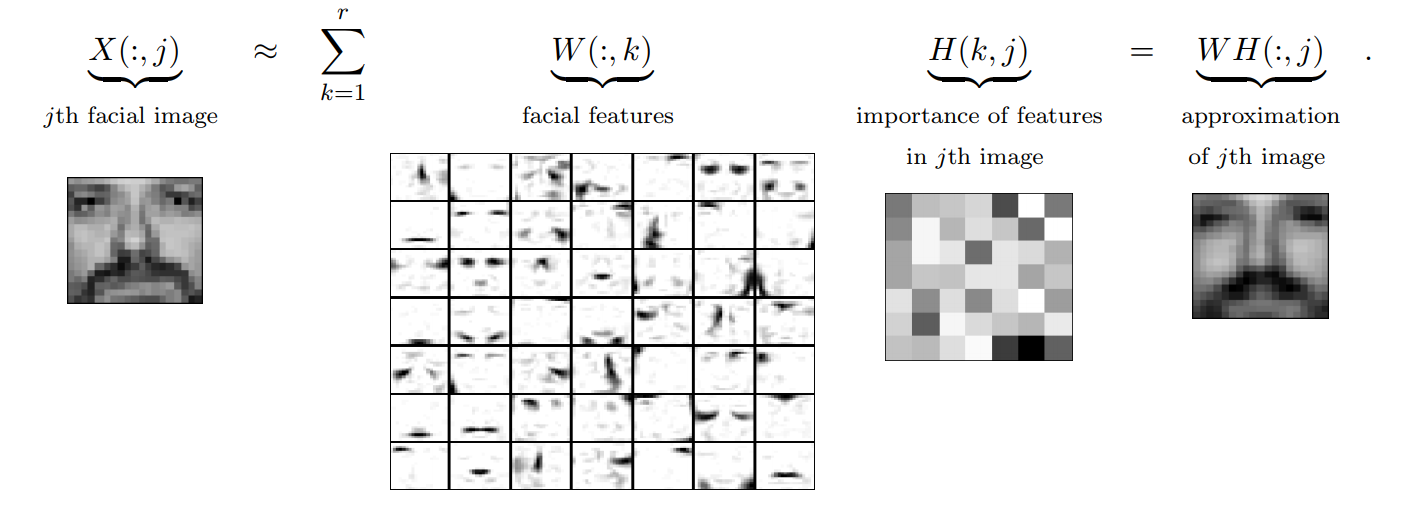
\includegraphics[width=0.9\textwidth]{face_decomp}
\caption{Decomposition of the CBCL face database, MIT Center For Biological and Computation Learning
(2429 gray-level 19-by-19 pixels images) using $r$ = 49.} 
\label{fig3}
\end{figure}
\FloatBarrier

In the case of facial images, the basis images are features such as eyes, noses, mustaches, and lips (see Figure \ref{fig3}) while the columns of $\mathbf{H}$ indicate which feature is present in which image \cite{93}. Thus, a major potential application of NMF is in face recognition. It has for example been observed that NMF is more robust to occlusion than PCA (which generates dense factors): in fact, if a new occluded face (e.g., with sun glasses) has to be mapped into the NMF basis, the non-occluded parts (e.g., the mustache or the lips) can still be well approximated.

\subsection{Action Recognition via Depth Silhouette Extraction}
NMF, is shown by \cite{action}, to be the most effective and accurate method for action/gesture recognition in images via depth silhouette extraction. NMF outperforms other methods such as PCA by over 9\%.

\FloatBarrier
\begin{wrapfigure}{l}{0.5\textwidth}
\begin{center}
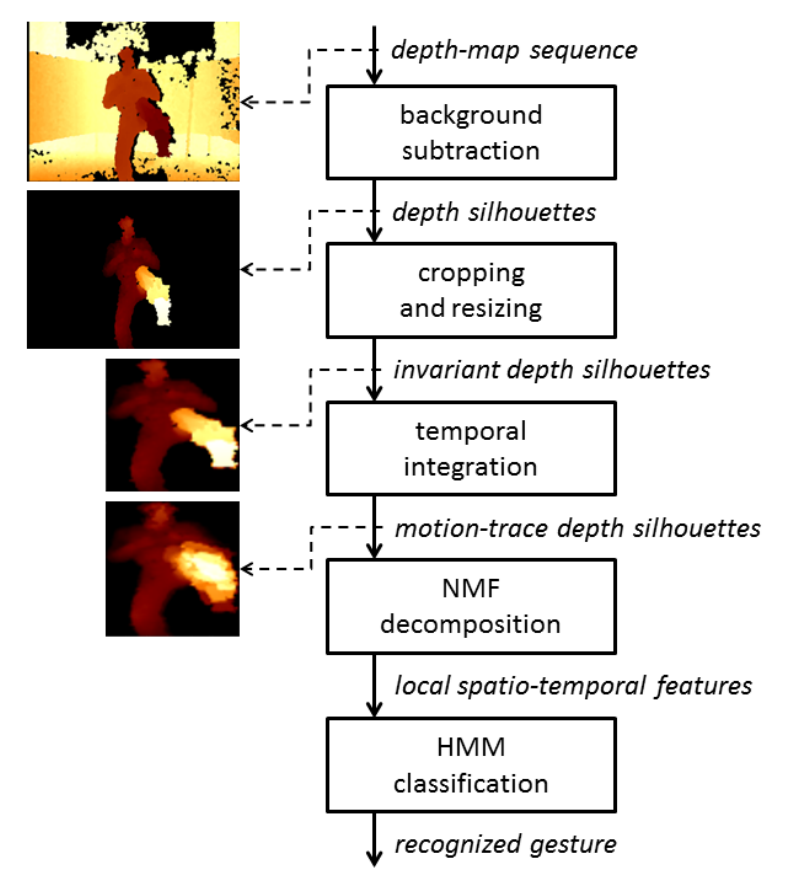
\includegraphics[width=0.4\textwidth]{gesture}
\end{center}
\caption{Schematic illustration of gesture recognition approach with NMF.} 
\label{fig4}
\end{wrapfigure}
\FloatBarrier

In the pipeline shown in Figure \ref{fig4} the motion-trace representation can be seen as a global representation of a short time instant of a full body gesture, and must be decomposed into local spatio-temporal patterns. NMF is known to be appropriate for representing an image as a linear combination of images parts which may be previously learned. Here the observation matrix $\mathbf{X}$ is formed by a concatenation of vectorized version of motion-traces. $\mathbf{W}$ is a dictionary of local spatio-temporal features and $\mathbf{H}$ represents the activations of each local motion feature for each respective motion-traces. $\mathbf{X}$, $\mathbf{W}$ and $\mathbf{H}$ have respectively the dimensions $F \times N$, $F \times K$ and $K \times N$ with $F$ the dimension of the vectorized motion-trace representation, $K$ the number of dictionary components and $N$ the number of motion-trace examples. $D_{SE}(x|y) = \frac{1}{2}(x-y)^2$ is used as divergence.

\section{Analysis and Conclusion} \label{analysis}

In this section we provide an analysis of the performance of the above discussed NMF algorithms based on numerical experiments on the dense CBCL data set (on the left, Figure \ref{fig5}), and the sparse Classic document data set (on the right, Figure \ref{fig5}), performed by \cite{p22}, \cite{f63}, \cite{f47}, and \cite{11}. 

\begin{figure}[ht!]
\begin{center}
\begin{tabular}{cc}
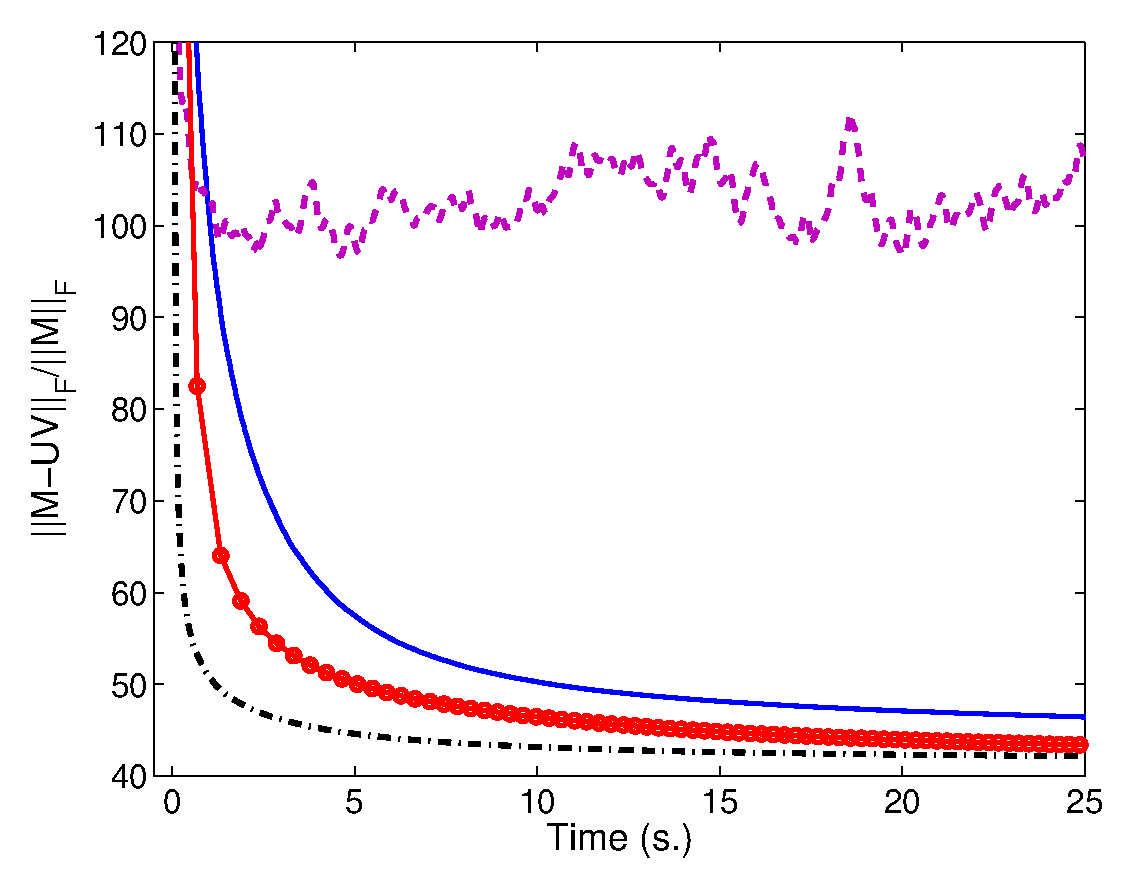
\includegraphics[width=8cm]{cbcl.eps}  & 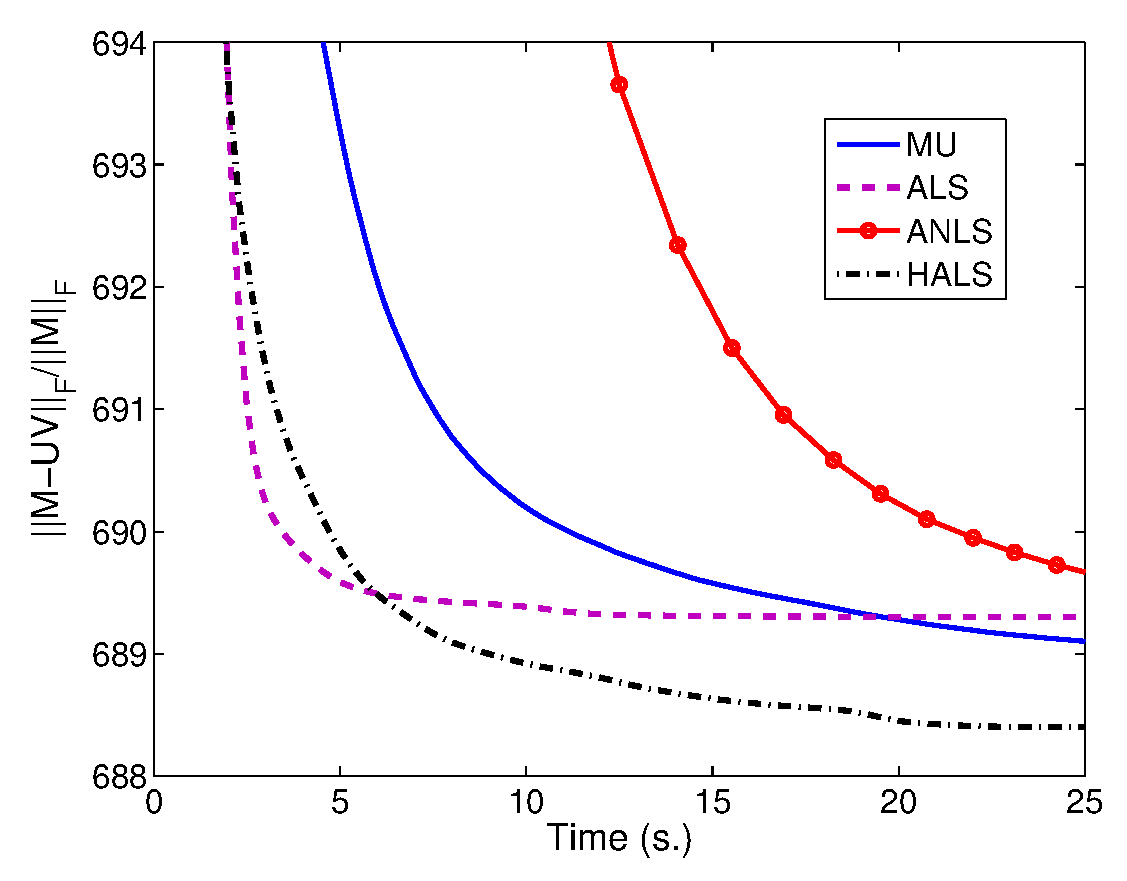
\includegraphics[width=8cm]{classic.eps}  \\
\end{tabular}
\end{center} 
\caption{\small Comparison of MU, ALS, ANLS and HALS. On the left: CBCL facial images with $r=49$; On the right: Classic document data set with $m=7094$, $n = 41681$ and $r= 20$. The figure displays the average error using the same ten initial matrices $W$ and $H$ for all algorithms, randomly generated with the \texttt{rand} function of Matlab. For MU and HALS, we used the implementation from \protect\url{https://sites.google.com/site/nicolasgillis/}, for ANLS and ALS from \protect\url{http://www.cc.gatech.edu/~hpark/nmfsoftware.php}. All tests and numerical evaluations discussed here are based on experiments performed using Matlab by \protect\cite{f47}}
\label{fig5}
\end{figure} 
\newpage
As anticipated from the theoretical background and above discussed mathematics of the different algorithms in the previous sections, we see that:
\begin{itemize}
\item The MU converge rather slowly.
\item ALS oscillates for the dense matrix (CBCL data set) and performs quite poorly while, for the
sparse matrix (Classic data set), it converges initially very fast but then stabilizes and cannot
compute a solution with small objective function value.
\item ANLS performs rather well for the dense matrix and is the second best after HALS. However,
it performs rather poorly for the sparse matrix.
\item HALS performs the best as it generates the best solutions within an allotted time.\\
\end{itemize}

In conclusion, NMF is an easily interpretable linear dimensionality reduction technique for nonnegative data. It is a rather versatile technique with many applications, and brings together a broad range of researchers. In the context of big data and data science, which is continuing to become an increasingly important topic. Further research on NMF includes the design of more efficient algorithms, in particular for regularized problems.


%%%%%%%%%%%%%%%%%%%%%%%%%%%%%%%%%%%%%%%%%%%%%%%%
%%%%%%%%%%%%%%%%%%%%%%%%%%%%%%%%%%%%%%%%%%%%%%%%
\bibliographystyle{acl}
\bibliography{coling2016}

\begin{thebibliography}{}

\bibitem[\protect\citename{Lee, Daniel D., and H. Sebastian Seung}1999]{93}
Lee, Daniel D., and H. Sebastian Seung.
\newblock {\em Learning of the parts of objects by non-negative matrix factorization.}
\newblock Nature 401.6755 (1999): 788.

\bibitem[\protect\citename{Lee, Daniel D., and H. Sebastian Seung}2001]{94}
Lee, Daniel D., and H. Sebastian Seung.
\newblock {\em Algorithms for Nonnegative Matrix Factorization.}
\newblock Advances in neural information processing systems (NIPS). 2001.

\bibitem[\protect\citename{Berry, Michael W., M. Browne, A. Langville, P. Pauca, and R. Plemmons}2007]{11}
Berry, Michael W., M. Browne, A. Langville, P. Pauca, and R. Plemmons.
\newblock {\em Algorithms and applications for approximate nonnegative matrix factorization.}
\newblock Computational statistics and data analysis 52.1 (2007): 155-173.

\bibitem[\protect\citename{Cichocki, Andrzej, Rafal Zdunek, and Shun-ichi Amari}2006]{35}
Cichocki, Andrzej, Rafal Zdunek, and Shun-ichi Amari.
\newblock {\em Csiszar’s divergences for non-negative matrix factorization: Family of new algorithms.}
\newblock International Conference on Independent Component Analysis and Signal Separation. Springer, Berlin, Heidelberg, 2006.

\bibitem[\protect\citename{Sra, Suvrit, and Inderjit S. Dhillon}2006]{49}
Sra, Suvrit, and Inderjit S. Dhillon.
\newblock {\em Generalized nonnegative matrix approximations with Bregman divergences.}
\newblock Advances in neural information processing systems (NIPS). 2006.

\bibitem[\protect\citename{Ding, Chris, Tao Li, Wei Peng, and Haesun Park}2006]{52}
Ding, Chris, Tao Li, Wei Peng, and Haesun Park.
\newblock {\em Orthogonal nonnegative matrix t-factorizations for clustering.}
\newblock  Proceedings of the 12th ACM SIGKDD international conference on Knowledge discovery and data mining. ACM, 2006.

\bibitem[\protect\citename{Dong, Bo, Matthew M. Lin, and Moody T. Chu}2008]{53}
Dong, Bo, Matthew M. Lin, and Moody T. Chu.
\newblock {\em Nonnegative rank factorization via rank reduction.}
\newblock http://www4.ncsu.edu/ mtchu/Research/Papers/Readme.html, page (preprint), 2008.

\bibitem[\protect\citename{Kolda, Tamara G., and Brett W. Bader}2009]{85}
Kolda, Tamara G., and Brett W. Bader.
\newblock {\em Tensor decompositions and applications.}
\newblock SIAM International Conference on Data Mining (SDM) review, 51(3) (2009): 455-500.

\bibitem[\protect\citename{Paatero, Pentti, and Unto Tapper}1994]{113}
Paatero, Pentti, and Unto Tapper. 
\newblock {\em Positive matrix factorization: A nonnegative factor model with optimal utilization of error estimates of data values.}
\newblock Environmetrics 5.2 (1994): 111-126.

\bibitem[\protect\citename{Hasan, Milos, Fabio Pellacini, and Kavita Bala}2007]{66}
Hasan, Milos, Fabio Pellacini, and Kavita Bala. 
\newblock {\em Matrix row-column sampling for the many-light problem.}
\newblock ACM Transactions on Graphics (TOG). Vol. 26. No. 3. ACM, 2007.

\bibitem[\protect\citename{Boutsidis, Christos, Michael W. Mahoney, and Petros Drineas}2009]{15}
Boutsidis, Christos, Michael W. Mahoney, and Petros Drineas.
\newblock {\em An improved approximation algorithm for the column subset selection problem.}
\newblock Proceedings of the 20th annual ACM-SIAM symposium on Discrete algorithms. Society for Industrial and Applied Mathematics, 2009.

\bibitem[\protect\citename{Kim, Jingu, Yunlong He, and Haesun Park}2014]{1}
Kim, Jingu, Yunlong He, and Haesun Park.
\newblock {\em Algorithms for nonnegative matrix and tensor factorizations: A unified view based on block coordinate descent framework.}
\newblock Journal of Global Optimization 58.2 (2014): 285-319.

\bibitem[\protect\citename{Bellavia, Stefania, Maria Macconi, and Benedetta Morini}2006]{p2}
Bellavia, Stefania, Maria Macconi, and Benedetta Morini.
\newblock {\em An interior point Newton‐like method for non‐negative least‐squares problems with degenerate solution.}
\newblock Numerical Linear Algebra with Applications 13.10 (2006): 825-846.

\bibitem[\protect\citename{Chu, Moody T., and Matthew M. Lin}2008]{p18}
Chu, Moody T., and Matthew M. Lin.
\newblock {\em Low-dimensional polytope approximation and its applications to nonnegative matrix factorization.}
\newblock SIAM Journal on Scientific Computing 30.3 (2008): 1131-1155.

\bibitem[\protect\citename{Cichocki, Andrzej, et al}2009]{p22}
Cichocki, Andrzej, et al.
\newblock {\em Nonnegative matrix and tensor factorizations: applications to exploratory multi-way data analysis and blind source separation.}
\newblock John Wiley and Sons, 2009.

\bibitem[\protect\citename{Gillis, Nicolas}2011]{f47}
Gillis, Nicolas.
\newblock {\em Nonnegative matrix factorization: Complexity, algorithms and applications.}
\newblock Doctoral dissertation, Universite catholique de Louvain. Louvain-La-Neuve: CORE (2011).

\bibitem[\protect\citename{Kim, Hyunsoo, and Haesun Park}2008]{500}
Kim, Hyunsoo, and Haesun Park.
\newblock {\em Nonnegative matrix factorization based on alternating nonnegativity constrained least squares and active set method.}
\newblock SIAM journal on matrix analysis and applications 30.2 (2008): 713-730.

\bibitem[\protect\citename{Ho, Ngoc-Diep}2008]{f63}
Ho, Ngoc-Diep.
\newblock {\em Nonnegative matrix factorization algorithms and applications.}
\newblock PhD thesis, Universite catholique de Louvain, 2008.

\bibitem[\protect\citename{Li, Liangda, Guy Lebanon, and Haesun Park}2012]{g83}
Li, Liangda, Guy Lebanon, and Haesun Park.
\newblock {\em Fast Bregman divergence NMF using Taylor expansion and coordinate descent.}
\newblock Proceedings of the 18th ACM SIGKDD international conference on Knowledge discovery and data mining. ACM, 2012.

\bibitem[\protect\citename{Franc, Vojtech, Vaclav Hlavac, and Mirko Navara}2005]{p31}
Franc, Vojtech, Vaclav Hlavac, and Mirko Navara.
\newblock {\em Sequential coordinate-wise algorithm for the non-negative least squares problem.}
\newblock CAIP. Vol. 3691. 2005.

\bibitem[\protect\citename{Moitra, Ankur}2013]{500}
Moitra, Ankur.
\newblock {\em An almost optimal algorithm for computing nonnegative rank.}
\newblock SIAM Journal on Computing 45.1 (2016): 156-173.

\bibitem[\protect\citename{Liu, Tongliang, Mingming Gong, and Dacheng Tao}2017]{500}
Liu, Tongliang, Mingming Gong, and Dacheng Tao.
\newblock {\em Large-cone nonnegative matrix factorization.}
\newblock IEEE transactions on neural networks and learning systems (2017).

\bibitem[\protect\citename{Vandaele, Arnaud, Nicolas Gillis, François Glineur, and Daniel Tuyttens}2016]{500}
Vandaele, Arnaud, Nicolas Gillis, François Glineur, and Daniel Tuyttens.
\newblock {\em Heuristics for exact nonnegative matrix factorization.}
\newblock SJournal of Global Optimization 65.2 (2016): 369-400.


\bibitem[\protect\citename{Masurelle, Aymeric, Slim Essid, and Gaël Richard}2014]{action}
Masurelle, Aymeric, Slim Essid, and Gaël Richard.
\newblock {\em Gesture recognition using a NMF-based representation of motion-traces extracted from depth silhouettes.}
\newblock Acoustics, Speech and Signal Processing (ICASSP), 2014 IEEE International Conference on. IEEE, 2014.

\bibitem[\protect\citename{Gillis, Nicolas}2014]{5000}
Gillis, Nicolas.
\newblock {\em The why and how of nonnegative matrix factorization.}
\newblock Regularization, Optimization, Kernels, and Support Vector Machines 12.257 (2014).

\bibitem[\protect\citename{Daube-Witherspoon, Margaret E., and Gerd Muehllehner}1986]{DM86}
Daube-Witherspoon, Margaret E., and Gerd Muehllehner.
\newblock {\em An iterative image space reconstruction algorthm suitable for volume ECT.}
\newblock IEEE transactions on medical imaging 5.2 (1986): 61-66.

\bibitem[\protect\citename{Yang, Jaewon, and Jure Leskovec}2013]{5000}
Daube-Witherspoon, Margaret E., and Gerd Muehllehner.
\newblock {\em Overlapping community detection at scale: a nonnegative matrix factorization approach.}
\newblock Proceedings of the sixth ACM international conference on Web search and data mining. ACM, 2013.

\bibitem[\protect\citename{Yang, Zhirong, and Erkki Oja}2010]{500}
Yang, Zhirong, and Erkki Oja.
\newblock {\em Linear and nonlinear projective nonnegative matrix factorization.}
\newblock IEEE Transactions on Neural Networks 21.5 (2010): 734-749.

\bibitem[\protect\citename{Donoho, David, and Victoria Stodden}2004]{p27}
Donoho, David, and Victoria Stodden.
\newblock {\em When does non-negative matrix factorization give a correct decomposition into parts?.}
\newblock Advances in neural information processing systems (NIPS). 2004.

\bibitem[\protect\citename{Sandler, Roman, and Michael Lindenbaum}2009]{500}
Sandler, Roman, and Michael Lindenbaum.
\newblock {\em Nonnegative matrix factorization with earth mover's distance metric.}
\newblock Computer Vision and Pattern Recognition, 2009. CVPR 2009. IEEE Conference on. IEEE, 2009.


\end{thebibliography}

\end{document}
